\documentclass[12pt]{article}\usepackage{graphicx, color}
%% maxwidth is the original width if it is less than linewidth
%% otherwise use linewidth (to make sure the graphics do not exceed the margin)
\makeatletter
\def\maxwidth{ %
  \ifdim\Gin@nat@width>\linewidth
    \linewidth
  \else
    \Gin@nat@width
  \fi
}
\makeatother

\IfFileExists{upquote.sty}{\usepackage{upquote}}{}
\definecolor{fgcolor}{rgb}{0.2, 0.2, 0.2}
\newcommand{\hlnumber}[1]{\textcolor[rgb]{0,0,0}{#1}}%
\newcommand{\hlfunctioncall}[1]{\textcolor[rgb]{0.501960784313725,0,0.329411764705882}{\textbf{#1}}}%
\newcommand{\hlstring}[1]{\textcolor[rgb]{0.6,0.6,1}{#1}}%
\newcommand{\hlkeyword}[1]{\textcolor[rgb]{0,0,0}{\textbf{#1}}}%
\newcommand{\hlargument}[1]{\textcolor[rgb]{0.690196078431373,0.250980392156863,0.0196078431372549}{#1}}%
\newcommand{\hlcomment}[1]{\textcolor[rgb]{0.180392156862745,0.6,0.341176470588235}{#1}}%
\newcommand{\hlroxygencomment}[1]{\textcolor[rgb]{0.43921568627451,0.47843137254902,0.701960784313725}{#1}}%
\newcommand{\hlformalargs}[1]{\textcolor[rgb]{0.690196078431373,0.250980392156863,0.0196078431372549}{#1}}%
\newcommand{\hleqformalargs}[1]{\textcolor[rgb]{0.690196078431373,0.250980392156863,0.0196078431372549}{#1}}%
\newcommand{\hlassignement}[1]{\textcolor[rgb]{0,0,0}{\textbf{#1}}}%
\newcommand{\hlpackage}[1]{\textcolor[rgb]{0.588235294117647,0.709803921568627,0.145098039215686}{#1}}%
\newcommand{\hlslot}[1]{\textit{#1}}%
\newcommand{\hlsymbol}[1]{\textcolor[rgb]{0,0,0}{#1}}%
\newcommand{\hlprompt}[1]{\textcolor[rgb]{0.2,0.2,0.2}{#1}}%

\usepackage{framed}
\makeatletter
\newenvironment{kframe}{%
 \def\at@end@of@kframe{}%
 \ifinner\ifhmode%
  \def\at@end@of@kframe{\end{minipage}}%
  \begin{minipage}{\columnwidth}%
 \fi\fi%
 \def\FrameCommand##1{\hskip\@totalleftmargin \hskip-\fboxsep
 \colorbox{shadecolor}{##1}\hskip-\fboxsep
     % There is no \\@totalrightmargin, so:
     \hskip-\linewidth \hskip-\@totalleftmargin \hskip\columnwidth}%
 \MakeFramed {\advance\hsize-\width
   \@totalleftmargin\z@ \linewidth\hsize
   \@setminipage}}%
 {\par\unskip\endMakeFramed%
 \at@end@of@kframe}
\makeatother

\definecolor{shadecolor}{rgb}{.97, .97, .97}
\definecolor{messagecolor}{rgb}{0, 0, 0}
\definecolor{warningcolor}{rgb}{1, 0, 1}
\definecolor{errorcolor}{rgb}{1, 0, 0}
\newenvironment{knitrout}{}{} % an empty environment to be redefined in TeX

\usepackage{alltt}
% !Rnw weave = knitr
% sweave fig help:
% http://users.stat.umn.edu/~geyer/Sweave/foo.pdf
% borrowing design from roxygen -- AJB Jan 13

%% \VignetteIndexEntry{DFT benchmarks: fft vs FFT.}
%% \VignetteEngine{knitr}

\usepackage[utf8]{inputenc}
\usepackage{fancyvrb}
\usepackage[pdfborder={0 0 0}]{hyperref}
\usepackage{url}
\usepackage{upquote}
\usepackage{graphicx}
\usepackage{grffile}
\usepackage{amsmath}
\usepackage{amssymb}
\usepackage{float}
\usepackage{natbib}
\usepackage{geometry}
\geometry{verbose,tmargin=3cm,bmargin=5cm,lmargin=2.5cm,rmargin=2.5cm}
%\usepackage{fullpage}
%captions
\usepackage[font=sf, labelfont={sf,bf}, margin=2cm]{caption}
\usepackage{makeidx} % for indexing
%\usepackage{showidx} % shows page (remove when complete)
\makeindex % comment to have no index
%%
%% Mathematics definitions
%% do not use special characters!
%%
%TMP\newcommand{\dxx}[1]{\enm{#1}} %% null
\newcommand{\enm}[1]{\ensuremath{#1}} %% null
\newcommand{\dFT}[0]{\enm{\mathfrak{F}}} %% fourier transform operator (FT)
\newcommand{\dFTp}[1]{\enm{\dFT{}\{#1\}}} %% FT{...}
\newcommand{\df}[0]{\enm{x}} %% stationary signal f
\newcommand{\dF}[0]{\enm{X}} %% FT{f}
\newcommand{\dmod}[1]{\enm{\mathrm{mod} \{#1\}}}
\newcommand{\dmodF}[0]{\dmod{\Xfo_T{}}}
\newcommand{\dargF}[0]{\enm{\mathrm{arg} \{ \Xfo_T{} \}}}
\newcommand{\ds}[0]{\enm{s}} %% spectrum
\newcommand{\dS}[0]{\enm{S(f)}} %% Spectrum
\newcommand{\dsupsf}[1]{\enm{{}^{#1}\ds{}}} %% superscript spectrum front
\newcommand{\dsupSf}[1]{\enm{{}^{#1}\dS{}}} %% superscript Spectrum front
\newcommand{\dsupsb}[1]{\enm{\ds{}^{#1}}} %% superscript spectrum back
\newcommand{\dsupSb}[1]{\enm{\dS{}^{#1}}} %% superscript Spectrum back
\newcommand{\daF}[0]{\enm{| \Xfo_T |}} %% amplitude Spectrum
\newcommand{\daS}[0]{\enm{\sqrt{\Re^2 + \Im^2}}} %% amplitude Spectrum
\newcommand{\dpS}[0]{\enm{\tan^{-1}\left(\Im / \Re \right)}} %% phase Spectrum
\newcommand{\dESD}[0]{\enm{E(f)}} %\dsupSf{\mathrm{(E)}}} %% energy Spectral density
\newcommand{\dPSD}[0]{\dsupSf{\mathrm{(P)}}} %% power Spectral density
%%
\newcommand{\intone}{\enm{\int_{- \infty} ^{\infty}}}
\newcommand{\Fo}{\enm{\mathcal{F}}}
\newcommand{\Xfo}{\enm{\tilde{X}}}
\newcommand{\stochXfo}{\enm{\tilde{\mathcal{X}}}}
\newcommand{\rXfo}{\enm{\Xfo{}^R}}
\newcommand{\iXfo}{\enm{\Xfo{}^I}}
\newcommand{\Ex}{\enm{\mathcal{E}}}
\newcommand{\slfrac}[2]{\left.#1\middle/#2\right.}
\newcommand{\half}{\enm{\slfrac{1}{2}}}
\newcommand{\nhalf}{\enm{\slfrac{-1}{2}}}
\newcommand{\Var}{\enm{\mathcal{V}}}
\newcommand{\Cov}{\enm{\mathrm{Cov}}}
\newcommand{\conv}{\ensuremath{\ast}}
%%
\newcommand{\dACV}[1]{\enm{\mathcal{R}(#1)}}
\newcommand{\dX}[1]{\enm{\mathcal{X}(#1)}}
\newcommand{\dXsub}[1]{\enm{\mathcal{X}_{#1}}}
\newcommand{\dXstoch}[0]{\dX{t}}
\newcommand{\dXstochd}[0]{\dXsub{n}}
\newcommand{\dXlag}[0]{\dX{\tau}}
\newcommand{\dXrealiz}[0]{\enm{X_T(t)}}
%%

%%
\newcommand{\SC}[1]{\textsc{#1}}
\newcommand{\SCY}[0]{\SC{Yes}}
\newcommand{\SCN}[0]{\SC{No}}
\newcommand{\Rcmd}[1]{\texttt{#1}}
\newcommand{\psd}[0]{\href{http://abarbour.github.com/psd/}{\color{blue}\Rcmd{psd}}}
\newcommand{\naive}[0]{na\"{\i}ve}
\newcommand{\bidx}[1]{\index{#1}{\textbf{#1}}} 
\newcommand{\idx}[1]{\index{#1}{#1}} 
%% path, filename, caption, label
\newcommand{\listing}[4]{        %
  \begin{figure}[H]              %
    \centering                   %
    \VerbatimInput[numbers=left, %
      frame=single,              %
      label=#2]{#1}              %
    \caption{#3}                 %
    \label{#4}                   %
  \end{figure}                   %
}
\author{Andrew J. Barbour}
\title{Benchmarks for Discrete Fourier Transforms in R}
\begin{document}
\maketitle
\begin{abstract}
The base DFT calculator in R, \Rcmd{stats::fft}, uses
the Mixed-Radix algorithm of \citet{singleton1969}.
In this vignette we show how 
this calculator compares
to \Rcmd{FFT} in the \Rcmd{fftw} package \citep{fftw}, which uses the
FFTW algorithm of \citet{frigo2005}.
For univariate DFT computations,
the methods are nearly equivalent with two exceptions which
are not mutually exclusive: 
(A) the series to be transformed is very long, and 
especially (B) when the series length is not highly composite.
In both exceptions the algorithm \Rcmd{FFT} outperforms \Rcmd{fft}.
\end{abstract}
\tableofcontents
\section{Benchmarking function}
We use both functions in their default state, and ask them
to transform the same univariate random series.
Benchmark information comes from the \Rcmd{rbenchmark}
program, and the versatile \Rcmd{plyr} and
\Rcmd{reshape2} packages are used to manipulate the information
for this presentation; \Rcmd{ggplot2} is used for plotting. 
First we load the libraries needed:
\begin{knitrout}
\definecolor{shadecolor}{rgb}{0.969, 0.969, 0.969}\color{fgcolor}\begin{kframe}
\begin{alltt}
\hlfunctioncall{rm}(list = \hlfunctioncall{ls}())
\hlfunctioncall{library}(fftw)
\hlfunctioncall{library}(rbenchmark)
\hlfunctioncall{library}(plyr)
\hlfunctioncall{library}(reshape2)
\hlfunctioncall{library}(ggplot2)
\end{alltt}
\end{kframe}
\end{knitrout}

and create a benchmark function:
\begin{knitrout}
\definecolor{shadecolor}{rgb}{0.969, 0.969, 0.969}\color{fgcolor}\begin{kframe}
\begin{alltt}
reps <- 10
dftbm <- \hlfunctioncall{function}(nd, repls = reps) \{
    \hlfunctioncall{set.seed}(1234)
    x <- \hlfunctioncall{rnorm}(nd, mean = 0, sd = 1)
    bmd <- \hlfunctioncall{benchmark}(replications = repls, fftw::\hlfunctioncall{FFT}(x), stats::\hlfunctioncall{fft}(x))
    bmd$num_dat <- nd
    bmd$relative[\hlfunctioncall{is.na}(bmd$relative)] <- 1  \hlcomment{# NA happens.}
    \hlfunctioncall{return}(bmd)
\}
\end{alltt}
\end{kframe}
\end{knitrout}


\section{Highly composite (HC) series}
It's well known that DFT algorithms are most efficient
for ``Highly Composite Numbers"\footnote{
This is the reason for the \Rcmd{stats::nextn} function.
}, specifically multiples of (2,3,5).

So, we create a vector of series lengths we wish to benchmark
\begin{knitrout}
\definecolor{shadecolor}{rgb}{0.969, 0.969, 0.969}\color{fgcolor}\begin{kframe}
\begin{alltt}
(nterms.even <- \hlfunctioncall{round}(2^\hlfunctioncall{seq.int}(from = 4, to = 20, by = 1)))
\end{alltt}
\begin{verbatim}
##  [1]      16      32      64     128     256     512    1024    2048
##  [9]    4096    8192   16384   32768   65536  131072  262144  524288
## [17] 1048576
\end{verbatim}
\end{kframe}
\end{knitrout}

and use it with \Rcmd{lapply} and the benchmark function
previously defined.
These data are further distilled into a usable format
with \Rcmd{ldply}:
\begin{knitrout}
\definecolor{shadecolor}{rgb}{0.969, 0.969, 0.969}\color{fgcolor}\begin{kframe}
\begin{alltt}
bench.even <- \hlfunctioncall{function}() \{
    benchdat.e <- plyr::\hlfunctioncall{ldply}(\hlfunctioncall{lapply}(X = nterms.even, FUN = dftbm))
\}
\hlfunctioncall{bench.even}()
\end{alltt}
\end{kframe}
\end{knitrout}


\section{Non highly composite (NHC) series}
DFT algorithms can have drastically reduced performance
if the series length is not highly composite (NHC).
We now test NHC series by adding one to the HC series-length
vector (also restricting the total length for sanity's sake):
\begin{knitrout}
\definecolor{shadecolor}{rgb}{0.969, 0.969, 0.969}\color{fgcolor}\begin{kframe}
\begin{alltt}
nterms.odd <- nterms.even + 1
nterms.odd <- nterms.odd[nterms.odd < 50000]  \hlcomment{# painfully long otherwise!}
\end{alltt}
\end{kframe}
\end{knitrout}

and performing the full set of benchmarks again:
\begin{knitrout}
\definecolor{shadecolor}{rgb}{0.969, 0.969, 0.969}\color{fgcolor}\begin{kframe}
\begin{alltt}
bench.odd <- \hlfunctioncall{function}() \{
    benchdat.o <- plyr::\hlfunctioncall{ldply}(\hlfunctioncall{lapply}(X = nterms.odd, FUN = dftbm))
\}
\hlfunctioncall{bench.odd}()  \hlcomment{# FAIR WARNING: this can take a while!!}
\end{alltt}
\end{kframe}
\end{knitrout}


\section{Visualization}
In order to plot the results, we need to 
perform some map/reduce operations on the data
\citep{wickham2010}. We intend to show faceted \Rcmd{ggplot2}-based
figures with row-wise summary information\footnote{
Based on this post:\\
{\small
\url{http://geokook.wordpress.com/2012/12/29/row-wise-summary-curves-in-faceted-ggplot2-figures/}
}
} so we can easily intercompare the benchmark data.
The benchmark data we will show
are \Rcmd{user.self}, \Rcmd{sys.self}, \Rcmd{elapsed}, and \Rcmd{relative}.
The results are shown
in Figure \ref{fig:results}.

\begin{knitrout}
\definecolor{shadecolor}{rgb}{0.969, 0.969, 0.969}\color{fgcolor}\begin{kframe}
\begin{alltt}
pltbench <- \hlfunctioncall{function}(lentyp=\hlfunctioncall{c}(\hlstring{"even"},\hlstring{"odd"}))\{
  benchdat <- \hlfunctioncall{switch}(\hlfunctioncall{match.arg}(lentyp), even=benchdat.e, odd=benchdat.o)
  \hlfunctioncall{stopifnot}(\hlfunctioncall{exists}(\hlstring{"benchdat"}))
  tests <- \hlfunctioncall{unique}(benchdat$test)
\hlcomment{  ## subset only information we care about}
  allbench.df.drp <- \hlfunctioncall{subset}(benchdat, 
        select=\hlfunctioncall{c}(test, num_dat, user.self, sys.self, elapsed, relative))
\hlcomment{  ## reduce data.frame with melt}
  allbench.df.mlt <- reshape2::\hlfunctioncall{melt}(allbench.df.drp, 
                                    id.vars=\hlfunctioncall{c}(\hlstring{"test"},\hlstring{"num_dat"}))
\hlcomment{  ## calculate the summary information to be plotted:}
  tmpd <- plyr::\hlfunctioncall{ddply}(allbench.df.mlt, 
                      \hlfunctioncall{.}(variable,  num_dat),
                      summarise, 
                      summary=\hlstring{"medians"}, # just a name
                      value=ggplot2::\hlfunctioncall{mean_cl_normal}(value)[1,1])
\hlcomment{  ## create copies for each test and map to data.frame}
  allmeds <<- plyr::\hlfunctioncall{ldply}(\hlfunctioncall{lapply}(X=tests, 
                                 FUN=\hlfunctioncall{function}(x,df=tmpd)\{
                                       df$test <- x; \hlfunctioncall{return}(df)
                                     \}))
\hlcomment{  ## plot the benchmark data}
  g <- \hlfunctioncall{ggplot}(data=allbench.df.mlt,
              \hlfunctioncall{aes}(x=\hlfunctioncall{log10}(num_dat),
                  y=\hlfunctioncall{log2}(value),
\hlcomment{                  # 1/sqrt(n) standard errors [assumes N(0,1)]}
                  ymin=\hlfunctioncall{log2}(value*(1-1/\hlfunctioncall{sqrt}(reps))),
                  ymax=\hlfunctioncall{log2}(value*(1+1/\hlfunctioncall{sqrt}(reps))),
                  colour=test,
                  group=test)) +
       \hlfunctioncall{scale_colour_discrete}(guide=\hlstring{"none"}) + 
       \hlfunctioncall{theme_bw}()+
       \hlfunctioncall{ylim}(\hlfunctioncall{c}(-11,11))+
       \hlfunctioncall{xlim}(\hlfunctioncall{c}(0.5,6.5))+
       \hlfunctioncall{ggtitle}(\hlfunctioncall{sprintf}(\hlstring{"DFT benchmarks of %s length series"},\hlfunctioncall{toupper}(lentyp)))
\hlcomment{  ## add previous summary curves if exist}
  \hlfunctioncall{if} (\hlfunctioncall{exists}(\hlstring{"allmeds.prev"}))\{
     g <- g + \hlfunctioncall{geom_path}(size=1.5, colour=\hlstring{"dark grey"}, data=allmeds.prev, 
                        \hlfunctioncall{aes}(group=test))
                        \}
\hlcomment{  ## create a facetted version}
  g2 <- g + \hlfunctioncall{facet_grid}(variable~test) #, scales=\hlstring{"free_y"})
\hlcomment{  ## add the summary data as a line}
  g3 <- g2 + \hlfunctioncall{geom_path}(colour=\hlstring{"black"}, data=allmeds, \hlfunctioncall{aes}(group=test))
\hlcomment{  ## and finally the data}
  \hlfunctioncall{print}(g4 <<- g3 + \hlfunctioncall{geom_pointrange}())
\}
\end{alltt}
\end{kframe}
\end{knitrout}


\begin{knitrout}
\definecolor{shadecolor}{rgb}{0.969, 0.969, 0.969}\color{fgcolor}\begin{kframe}
\begin{alltt}
\hlfunctioncall{pltbench}(\hlstring{"even"})
allmeds.prev <- allmeds
\hlfunctioncall{pltbench}(\hlstring{"odd"})
\end{alltt}
\end{kframe}
\end{knitrout}


\begin{figure}[htb!]
\begin{center}
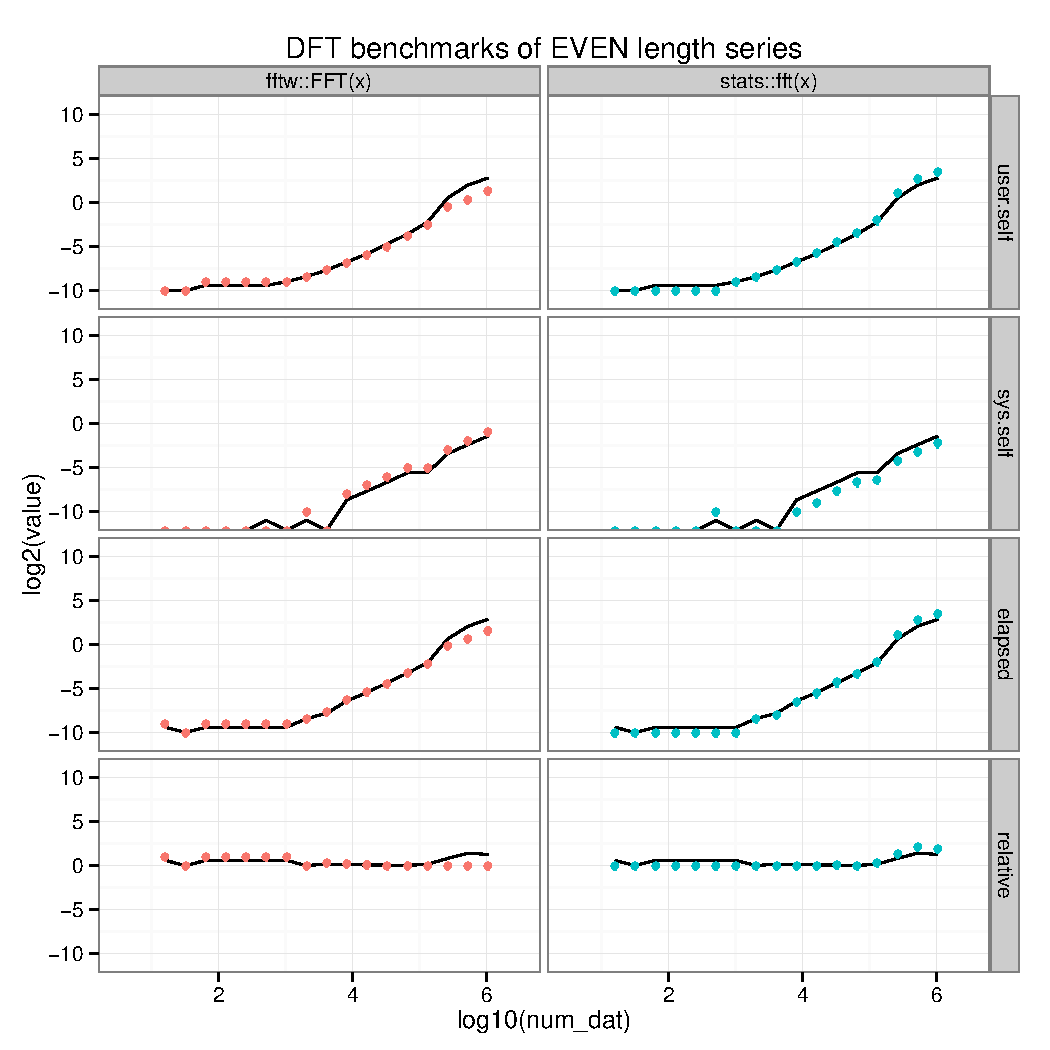
\includegraphics[width=0.5\textwidth]{fftw_bench_even}%
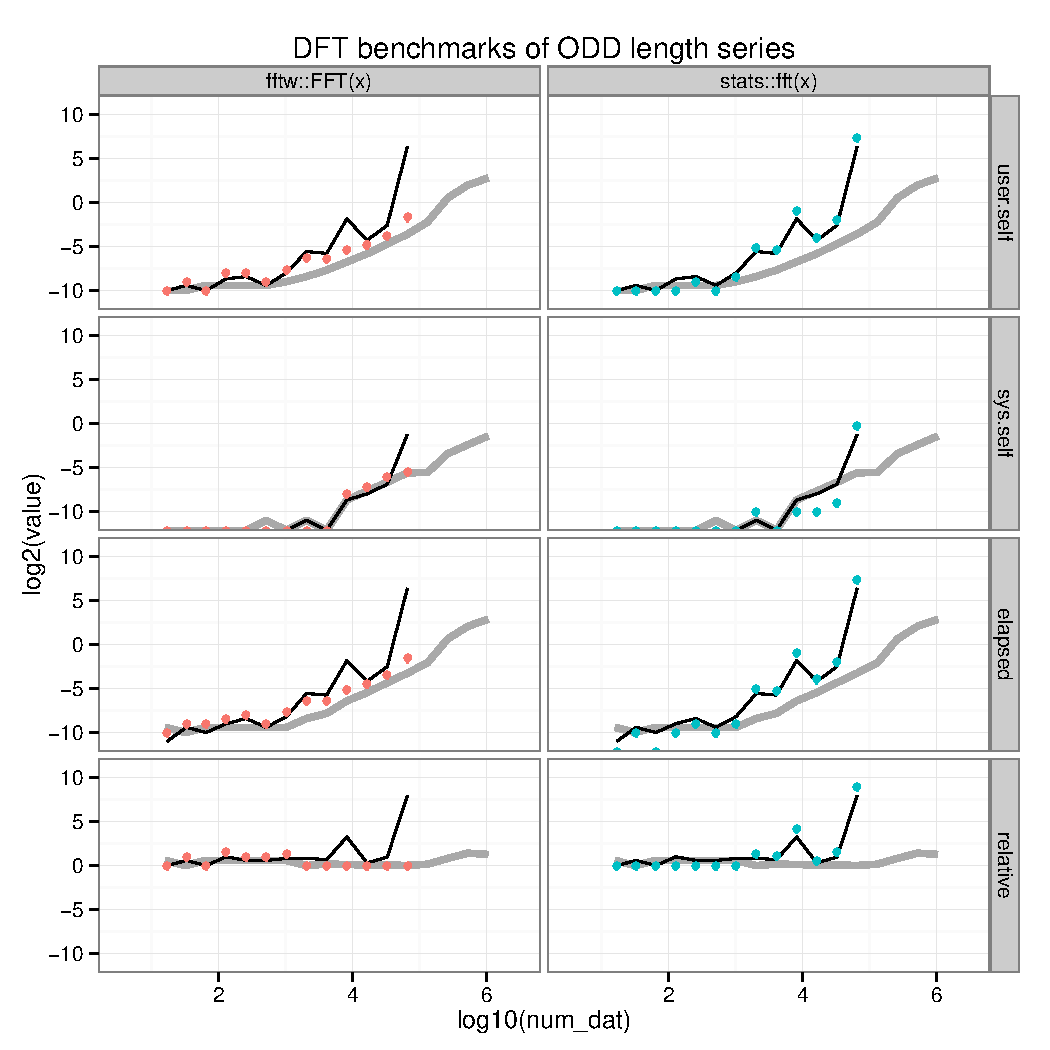
\includegraphics[width=0.5\textwidth]{fftw_bench_odd}
\caption{ DFT benchmark results for HC series lengths (left),
and NHC series lengths (right) as a function of logarithmic
series length.  In each figure, the left
facet-column is for results from \Rcmd{fftw::FFT} and the right
column is for \Rcmd{stats::fft}.
We also show the summary curves from the HC results
in the NHC frames (thick grey curve)
to highlight the drastic degradation in performance.}
\label{fig:results}
\end{center}
\end{figure}

\section{Conclusion}

Figure \ref{fig:results} compares the DFT
calculations for HC and NHC length series.
For univariate DFT computations,
the methods are nearly equivalent with two exceptions which
are not mutually exclusive: 
(A) the series to be transformed is very long, and 
especially (B) when the series length is not highly composite.
In both exceptions the algorithm \Rcmd{FFT} outperforms \Rcmd{fft}.
In the case of exception (B), both methods have
drastically increased computation times; hence, zero padding should be
done to ensure the length does not adversely
affect the efficiency of the DFT calculator.

\pagebreak

\section*{Session Info}
\begin{knitrout}
\definecolor{shadecolor}{rgb}{0.969, 0.969, 0.969}\color{fgcolor}\begin{kframe}
\begin{alltt}
\hlfunctioncall{sessionInfo}()
\end{alltt}
\begin{verbatim}
## R version 2.15.2 (2012-10-26)
## Platform: x86_64-apple-darwin9.8.0/x86_64 (64-bit)
## 
## locale:
## [1] C
## 
## attached base packages:
##  [1] parallel  datasets  grDevices grid      graphics  tools     stats    
##  [8] utils     methods   base     
## 
## other attached packages:
## [1] knitr_0.9
## 
## loaded via a namespace (and not attached):
## [1] digest_0.6.0   evaluate_0.4.3 formatR_0.7    stringr_0.6.2
\end{verbatim}
\end{kframe}
\end{knitrout}


%% bib and index
\bibliographystyle{apalike}
\bibliography{REFS}

\printindex
\end{document}
